\begin{figure}[t]
\centering
\begin{subfigure}[b]{0.475\columnwidth}
    \resizebox{\columnwidth}{!}{
        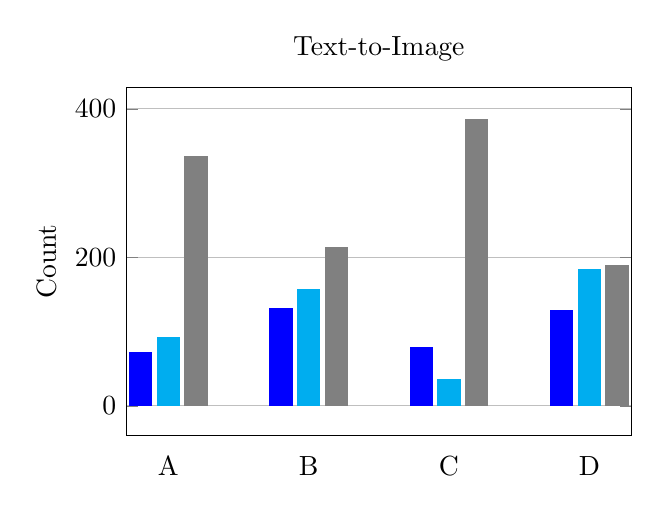
\begin{tikzpicture}
            \begin{axis}[
                major x tick style = transparent,
                ybar,
                bar width=8pt,
                ymajorgrids = true,
                width=8cm,height=6cm,
                title=Text-to-Image,
                % xlabel = Moderators,
                ylabel = Count,
                symbolic x coords={A,B,C,D},
                xtick = data,
                scaled y ticks = false,
                ymin = -40,
            ]
                \addplot[style={blue,fill=blue,mark=none}]
                    coordinates {(A,72) (B,131) (C,79) (D,128)};
        
                \addplot[style={cyan,fill=cyan,mark=none}]
                    coordinates {(A,92) (B,156) (C,35) (D,183)};
        
                \addplot[style={gray,fill=gray,mark=none}]
                    coordinates {(A,336) (B,213) (C,386) (D,189)};
                \end{axis}
        \end{tikzpicture}
    }
\end{subfigure}
\hfill
\begin{subfigure}[b]{0.475\columnwidth}
    \resizebox{\columnwidth}{!}{
        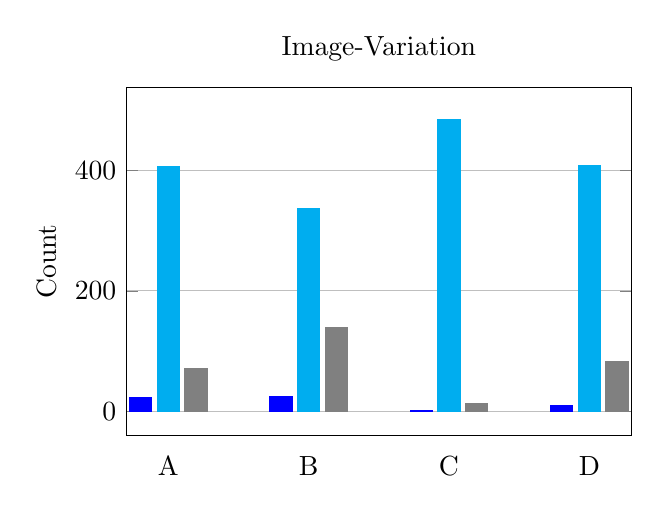
\begin{tikzpicture}
            \begin{axis}[
                major x tick style = transparent,
                ybar,
                bar width=8pt,
                ymajorgrids = true,
                width=8cm,height=6cm,
                title=Image-Variation,
                % xlabel = Moderators,
                ylabel = Count,
                symbolic x coords={A,B,C,D},
                xtick = data,
                scaled y ticks = false,
                ymin = -40,
            ]
                \addplot[style={blue,fill=blue,mark=none}]
                    coordinates {(A,23) (B,25) (C,2) (D,10)};
        
                \addplot[style={cyan,fill=cyan,mark=none}]
                    coordinates {(A,406) (B,336) (C,485) (D,408)};
        
                \addplot[style={gray,fill=gray,mark=none}]
                    coordinates {(A,71) (B,139) (C,13) (D,82)};
                \end{axis}
        \end{tikzpicture}
    }
\end{subfigure}
\caption{User studies on text-to-image and image-variation in which we count the votes from 4 individual moderators on SD (\textcolor{blue}{blue}), VD (\textcolor{cyan}{cyan}), or equally good (\textcolor{gray}{gray}).}
\vspace{-0.2cm}
\label{fig:user_study}
\end{figure}